\documentclass{llncs}

\usepackage[utf8]{inputenc}
%\usepackage{fancyvrb,amssymb,graphicx}
%\usepackage[usenames,dvipsnames,svgnames,table]{xcolor}

% the following package is optional:
\usepackage{latexsym} 

\usepackage{graphicx}
% \usepackage{caption}
\usepackage{subcaption}
\captionsetup{compatibility=false}

\usepackage{wrapfig}

\usepackage{amsmath}
\usepackage{xspace}
\usepackage{graphicx,url}
\usepackage{txfonts} % needed for \Diamondblack
\usepackage{color}
\usepackage{xcolor}

\usepackage{proof}

\usepackage{fancyvrb}
\newcommand{\red}[1]{\textcolor[rgb]{1,0,0}{#1}}
\newcommand{\blue}[1]{\textcolor[rgb]{0,0,1}{#1}}
\newcommand{\brown}[1]{\textcolor[rgb]{0.8,0.6,0.4}{#1}}

\newcommand{\Parameter}{\red{Parameter}}
\newcommand{\Ltac}{\red{Ltac}}
\newcommand{\Axiom}{\red{Axiom}}
\newcommand{\Lemma}{\red{Lemma}}
\newcommand{\Theorem}{\red{Theorem}}
\newcommand{\Definition}{\red{Definition}}
\newcommand{\Notation}{\blue{Notation}}
\newcommand{\Prop}{\blue{Prop}}
\newcommand{\Type}{\blue{Type}}
\newcommand{\llet}{\blue{let}}
\newcommand{\match}{\blue{match}}
\newcommand{\with}{\blue{with}}
\newcommand{\eend}{\blue{end}}
\newcommand{\iin}{\blue{in}}
\newcommand{\as}{\blue{as}}
\newcommand{\Require}{\blue{Require}}
\newcommand{\Import}{\blue{Import}}
\newcommand{\fforall}{\blue{forall}}
\newcommand{\fun}{\blue{fun}}
\newcommand{\Proof}{\blue{Proof}}
\newcommand{\Qed}{\blue{Qed}}
\newcommand{\Hint}{\blue{Hint}}
\newcommand{\com}[1]{\brown{#1}}
\newcommand{\bslash}{\symbol{92}}

\newcommand{\verbsize}{\scriptsize}


%\usepackage{modallogics}
\newcommand{\logic}[1]{\textbf{#1}\xspace}
\newcommand{\KB}{\logic{KB}}
\newcommand{\KFour}{\logic{K4}}
\newcommand{\KFourB}{\logic{K4B}}
\newcommand{\K}{\logic{K}}
\newcommand{\KT}{\logic{KT}}
\newcommand{\SFour}{\logic{S4}}
\newcommand{\SFive}{\logic{S5}}
\newcommand{\SFiveU}{\logic{S5\textsuperscript{U}}}

\newcommand{\imp}{{\rightarrow}}
\newcommand{\biimp}{\leftrightarrow}
\newcommand{\allq}{\forall}
\newcommand{\exq}{\exists}
\newcommand{\seq}{\vdash}

\newcommand{\Dia}{\Diamond} % possibly
\newcommand{\BlackBox}{\blacksquare}
\newcommand{\BlackDia}{\Diamondblack}

\newcommand{\NE}{\mathit{NE}}
\newcommand{\ess}[2]{#1\ \mathit{ess}\ #2}
\newcommand{\nec}{\Box}
\newcommand{\pos}{\Dia}




\begin{document}

\title{An Object-Logic Explanation for the Inconsistency in G\"odel's
  Ontological Theory (Extended Abstract)}
\author{Christoph Benzm\"uller\inst{1}\thanks{This work was supported by
    the German Research Foundation DFG grant BE2501/9-1,2} \and Bruno Woltzenlogel Paleo\inst{2} 
}

\institute{
 Freie Universit\"at Berlin, Berlin, Germany \\ \url{c.benzmueller@fu-berlin.de}
\and
 Australian National University, Canberra,  Australia \\ \url{bruno.wp@gmail.com}
}

\maketitle            



\begin{abstract}
  This paper discusses the 
  inconsistency in G\"odel's
  ontological argument. Despite the popularity of G\"odel's argument, this
  inconsistency remained unnoticed until 2013, 
  when it was detected automatically by the 
  higher-order theorem prover \textsc{Leo-II}. Complementing the meta-logic explanation for the inconsistency available in our IJCAI 2016 paper \cite{C55}, we present here a new purely object-logic explanation that does not rely on semantic argumentation.
  
  % (This extended abstract is mostly a shortened version of our IJCAI 2016 paper \cite{C55}, but the explanation of the inconsistency is more detailed here.)
\end{abstract}



\section{Introduction}\label{sec:introduction}
% Without exaggeration 
Kurt G\"{o}del's ontological
argument for the existence of God \cite{GoedelNotes,ScottNotes} is
amongst the most discussed formal proofs in modern literature. A rich
body of publications -- including very recent ones -- present,
discuss, assess, criticize, modify and improve G\"{o}del's original
work (see e.g.~Sobel~\cite{sobel2004logic} and Oppy~\cite{sep-ontological-arguments} and the
references therein). 

Scott's version of G\"odel's argument was automatically reconstructed
by higher-order automated theorem provers \cite{C40} and its
correctness was verified step-by-step in the \textsc{Coq} proof
assistant \cite{CSR}. To bridge the gap between higher-order logics
(HOL; cf.~\cite{andrewsSEP} and the references therein), as used by
these systems, and higher-order \emph{modal} logics (HOML;
cf.~\cite{homl} and the references therein), on which the ontological
argument argument, the logic embedding approach \cite{J23,C40} was
used.

However, G\"odel's original axioms, as used in his
manuscript \cite{GoedelNotes}, are inconsistent. This fact has
remained unnoticed to philosophers until 2013, 
when \textsc{Leo-II} \cite{J30} found a surprising refutation of the axioms.
In \cite{C55} we extracted from Leo-II's machine-oriented refutation an informal and human-oriented intuitive explanation for the inconsistency, and we reconstructed and
verified it in the \textsc{Isabelle} proof assistant. But that explanation relied on reasoning at the meta-logic (HOL) level, which was only possible because of the embedding. Here we complement that work with a purely object-logic (HOML) explanation, and we compare and formalize both explanations in the \textsc{Coq} proof assistant.

Applications of (first-order) theorem proving technology in
metaphysics were first reported by Fitelson, Oppenheimer and
Zalta~\cite{FitelsonZalta,oppenheimer11}. 
%Zalta also coined the term
%\textit{Computational Metaphysics}. 
Later on, Rushby~\cite{rushby13} used the \textsc{PVS} proof
assistant. Common to both works is a
significant amount of proof-hand-coding work as well as their focus on
a non-modal formalization of St. Anselm's simpler
and older ontological argument.


\begin{figure}\centering 
  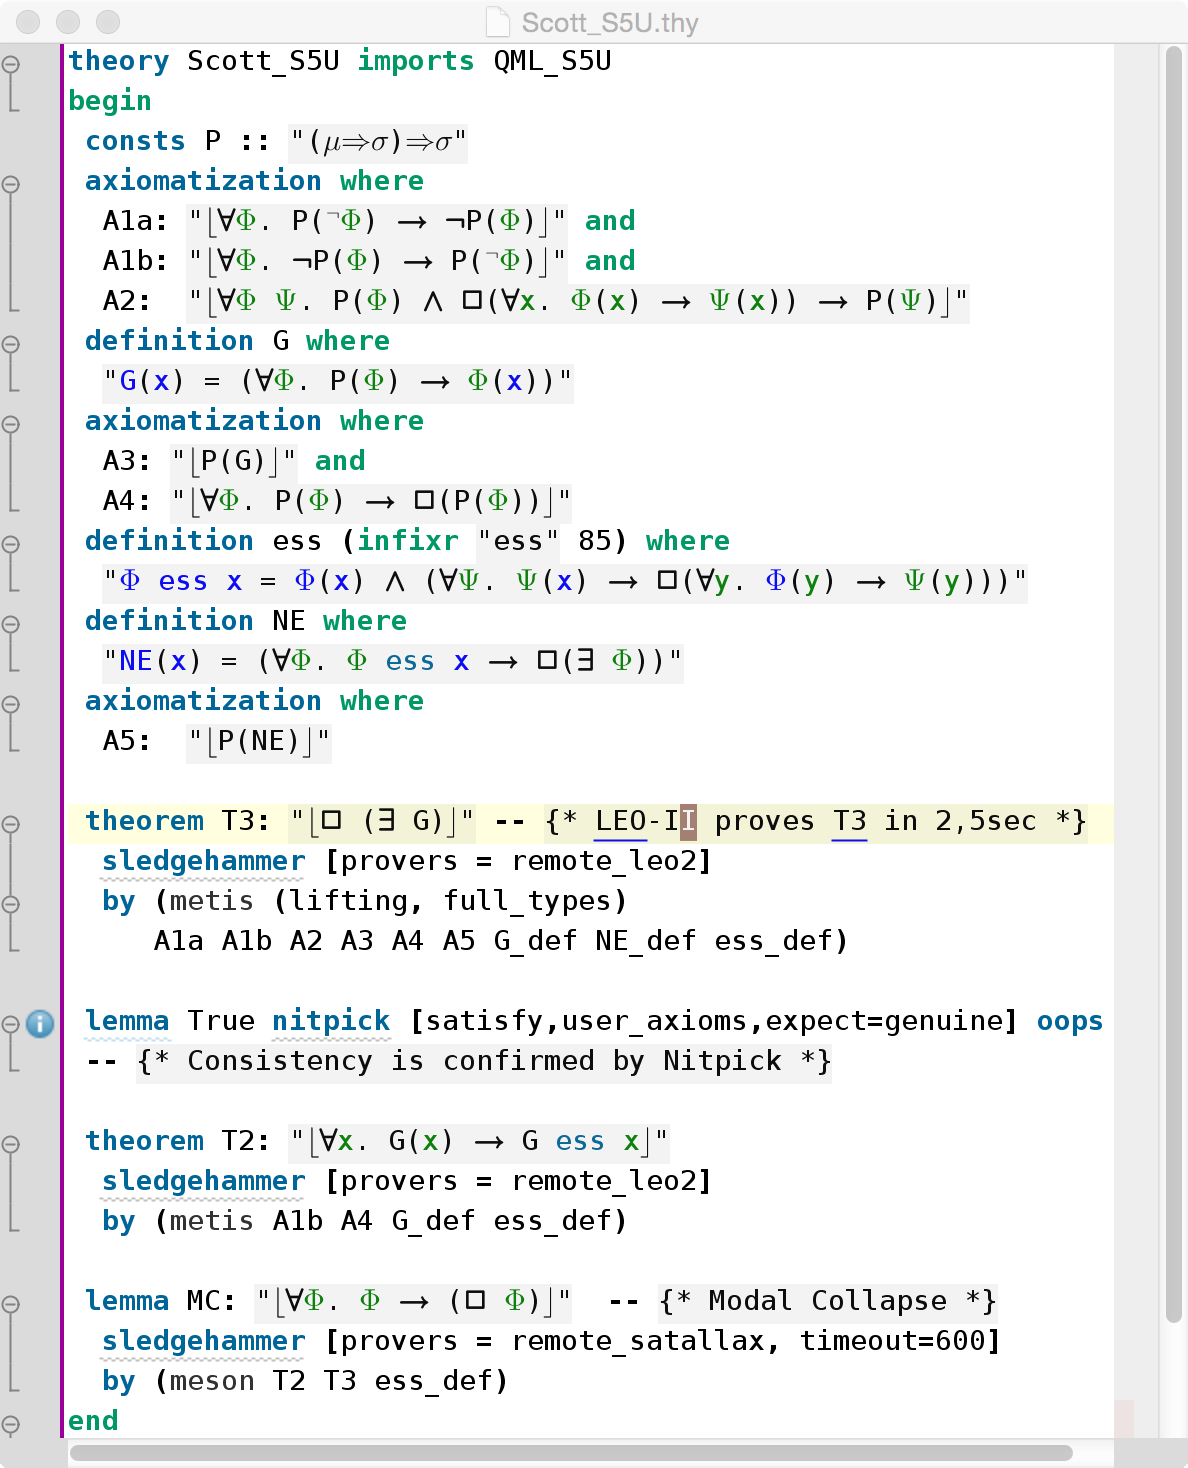
\includegraphics[width=.495\textwidth]{./Scott_S5U.png}
  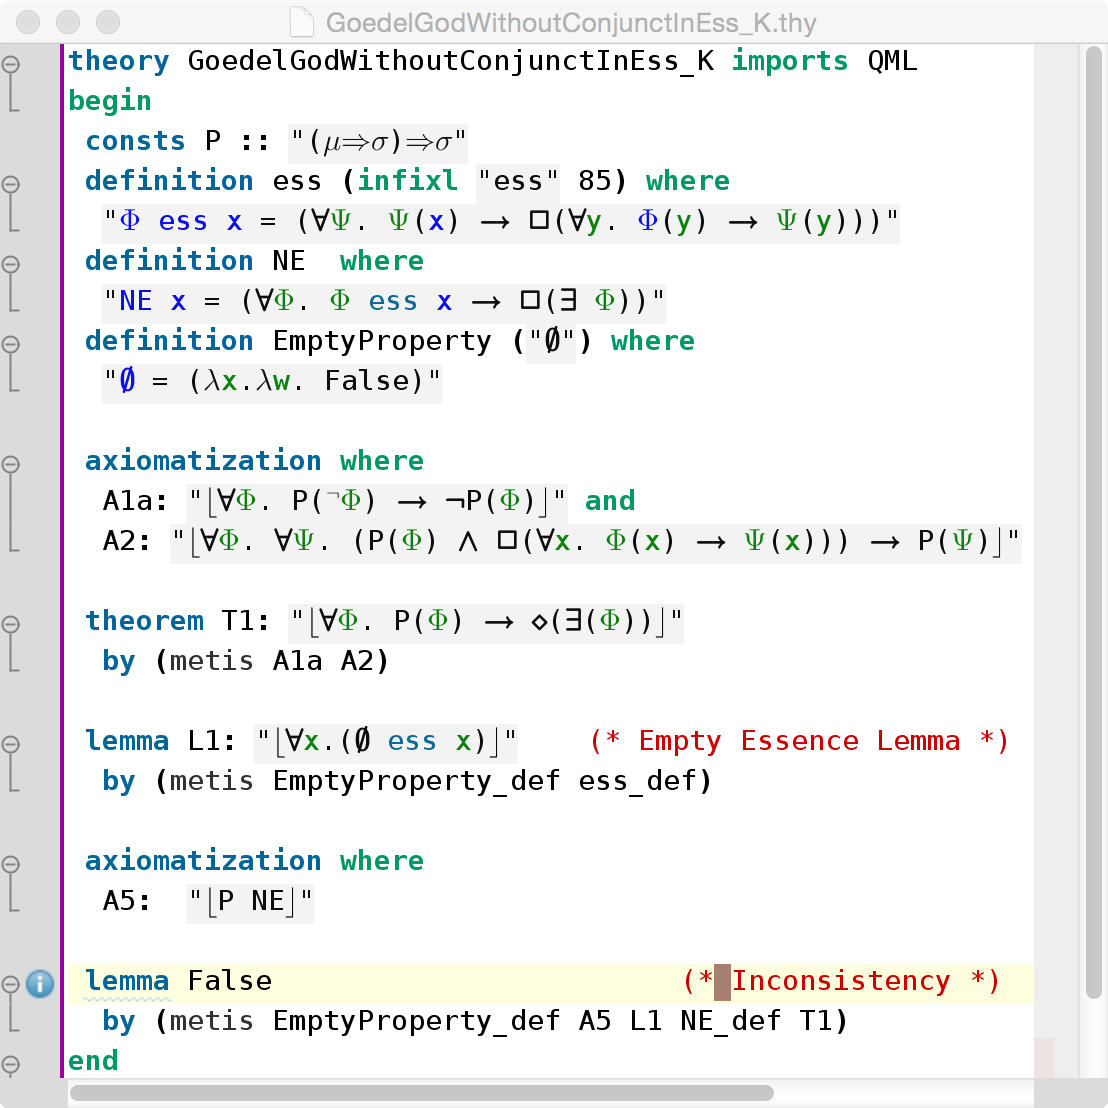
\includegraphics[width=.495\textwidth]{./InconsistencyIsabelleK.png}
  % \caption{Full Automation of T3 in \SFiveU; Consistency of Scott's
  % Axioms;  Automatic Verification of Modal Collapse} 
\caption{Scott's consistent axioms (left) and proof of the
  inconsistency of (a subset of) G\"odel's original  axioms (right)}
  % Axioms;  Automatic Verification of Modal Collapse} 
\label{Scott_Goedel}
\end{figure} 



\section{An Essential Difference in the Definitions of Essence.}
\label{sec:history}
G\"odel's manuscript can be considered a translation of Leibniz's
ideas on the argument into modern modal logic. G\"odel
discussed his manuscript with Scott, who shared a slightly different
version with a larger public. Scott's version of the axioms and
definitions, formalized in \textsc{Isabelle}, is shown in
Fig.~\ref{Scott_Goedel}. 
The main difference to G\"odel's version is an
extra conjunct in the definition of \emph{essence} (\emph{ess}). For Scott,
an essential property of an individual must be possessed by
him/her. For G\"odel, this is not required. 


G\"odel's omission has been
considered inessential and merely an oversight by many. 
For more than four decades, its serious consequences remained unnoticed, 
despite numerous analyses and criticisms of the
argument.
However, as explained here, the extra conjunct is in
fact crucial. Without it, G\"odel's original axioms are
inconsistent. With it, Scott's axioms are consistent (cf.~Fig.~\ref{Scott_Goedel},
where the model finder \textsc{Nitpick} \cite{Nitpick} confirms consistency). In
personal communication, Dana Scott confirmed that he was unaware
that G\"odel's original axioms were inconsistent.









\section{Automating HOML in HOL}\label{sec:homlinhol}



In our experiments in this branch of metaphysics we
utilise an embedding of HOMLs, such as \textbf{K}, \textbf{KB} and
\textbf{S5} with various domain conditions (possibilist and actualist
quantification), in HOL. More precisely, formulas in HOML are \emph{lifted}, i.e., converted
into predicates over worlds, which are themselves explicitly
represented as terms. The logical constants of HOML are translated to
HOL terms in such a way that, for instance,
%$\neg \varphi$, $\varphi\vee\psi$
$\Box \varphi$ and $\Diamond \varphi$ (relative to a current world
$w_0$) are mapped, respectively, to the HOL formulas
$\forall w. (r w_0 w) \imp (\varphi w)$ and
$\exists w. (r w_0 w) \wedge (\varphi w)$. This form of embedding is
precisely the well-known standard translation,
%\cite{DBLP:journals/logcom/Ohlbach91}, 
which is here intra-logically realized --- and extended for
quantifiers --- in HOL by stating a set of equations defining the
logical constants. The resulting object logic is
the HOML \textbf{K} with rigid terms and constant domains (possibilist
quantifiers). Other logics (e.g. \textbf{KB}, \textbf{S5}) are
embedded by adding axioms that restrict the accessibility relation
$r$. Varying domains and actualist quantifiers can be simulated by
using an existence predicate to guard the quantifiers. 



\section{Intuitive Explanations for the Inconsistency} 
\label{sec:inconsistency}

In the typical workflow during an attempt to prove a conjecture with a
theorem prover, it is customary to check the consistency of the axioms
first. For if the axioms are inconsistent, anything (including the
conjecture) would be trivially derivable in classical logic (\emph{ex
  falso quodlibet}). Surprisingly, when this routine check was
performed on G\"odel's axioms \cite{C40}, the \textsc{Leo-II} prover
claimed that the axioms were inconsistent. Unfortunately, the
refutation generated by \textsc{Leo-II} was barely human-readable. The
refutation was based on machine-oriented inference rules (a higher-order resolution calculus \cite{J30}), and the
text file had 153 lines (with an average of 184
  characters per line) and used a machine-oriented syntax (TPTP THF
\cite{J22}). 


Although \textsc{Leo-II}'s resolution refutation is not easy to read
for humans, it did contain relevant hints to the importance of the
empty property\footnote{
  Note that the terms for the empty property ($\lambda x. \bot$) and for the property of self-difference ($\lambda x.  x\not=x$) have identical denotations in the logic setting
  with functional and Boolean extensionality assumed
  here. 
  For the proof to go through it is
  irrelevant which property is used.
} $\lambda x. \bot$ (also denoted $\emptyset$, as in HOL it is customary to think of unary predicates as sets)\footnote{An additional lambda abstraction occurs in the empty property in \textsc{Leo-II}'s proof (and in the reconstruction in \textsc{Isabelle}) because the embedding approach lifts the boolean type $o$ to $\iota \imp o$.}. Based on this hint, we conceived the following informal explanation for the inconsistency of G\"odel's axioms (reproduced without change from \cite{C55}):
%


\begin{enumerate}
\item From G\"odel's definition of essence 
(${\ess{\phi}{x} \biimp {\allq \psi} (\psi(x)
\imp {\nec} \allq y (\phi(y) \imp \psi(y)))}$) it follows that the
empty property (or self-difference) is an essence of every individual
(\textbf{Empty Essence Lemma}): \hfill $\allq x\; (\ess{\emptyset}{x})$

\item From axiom A5 (`necessary existence' is a positive
  property: $P(\NE)$ ) and theorem T1 (\textit{Positive properties are possibly
  exemplified}: ${\allq \phi} [P(\phi) \imp {\pos}  \exq x
  \phi(x)]$), it follows that $\NE$ is possibly exemplified:
  \hfill $  \pos \exq x [\NE(x)] $
 
\item Expanding the definition of `necessary existence'
  (${\NE(x) \equiv \allq \phi [\ess{\phi}{x} \imp \nec \exq y
    \phi(y)]}$), the following is obtained: \hfill $  \pos \exq x
  [\allq \varphi [ \ess{\varphi}{x} \imp \nec \exq y [\varphi(y)] ] ] $

\item The sentence above holds for all $\varphi$ and thus, in
  particular, for the empty property (or self-difference): \hfill $\pos \exq x [ \ess{\emptyset}{x} \imp \nec \exq y [\emptyset(y)] ]$

\item By the Empty Essence Lemma, the antecedent of the implication
  above is valid. Therefore, the sentence above entails: \hfill $\pos \exq x [ \nec \exq y [\emptyset(y)] ]$ 

\item By definition of $\emptyset$: \hfill $\pos \exq x [ \nec \bot ]$

\item As the existential quantifier is binding no variable within its
  scope, the sentence is equi-valid with: \hfill $\pos \nec \bot $

\item To see that the sentence above is contradictory, we may reason semantically, thinking of possible worlds. If $w_0$ is the arbitrary current world, the $\pos$ operator forces the existence of a world $w$ accessible from $w_0$ such that $\nec \bot$ is true in $w$. But $\nec \bot$ can only be true in $w$, if there is no world $w'$ accessible from $w$. In logics\footnote{
  Interestingly, the refutation automatically generated by
  \textsc{Leo-II} uses a symmetric accessibility relation, and thus
  requires the modal logic \KB. The informal, human-constructed
  refutations described here, on the other hand, requires only the
  weaker modal logic \K. In our experiments \textsc{Leo-II} (like all
  other HOL provers) was still too weak to automatically prove the
  inconsistency already in logic \K. Hence, this remains an open problem for automated
  theorem provers.
} with a reflexive or symmetric accessibility relation (e.g. \KB), it is easy to see that there must be a world $w'$ accessible from $w$: either $w'$ itself, in case of a reflexive relation, or $w_0$, in case of a symmetric relation. In fact, even in \K, with no accessibility condition, there must be a world $w'$ accessible from $w$. The reason is that $\pos \nec \bot$ should be \emph{valid} (true in all worlds). Therefore, it is true in $w$ as well, where the existence of an accessible world $w'$ is forced by the $\pos$ operator. As a model for $\pos \nec \bot$ (which is a consequence of G\"odel's axioms) cannot be built, G\"odel's axioms are inconsistent.
\end{enumerate}

If we were to convert the informal proof above to a formal proof, the semantic reasoning in step 8 would require a leap to the meta-logic (HOL), in order to expand the definitions of the modal operators and reason directly about possible worlds. The following alternative proof avoids this leap and remains purely within the object logic (HOML \K):

\begin{enumerate}
\item[8\textsuperscript{*}.] We must derive $\bot$ from $\pos \nec \bot$. In order to derive $\bot$, it suffices to show that there exists a derivable proposition such that its negation is also derivable. We choose $\pos \pos \bot$ as a candidate proposition, and hence we must show that:
\begin{enumerate}
\item $\neg \pos \pos \bot$ \emph{is derivable:} this proposition is equi-valid to $\nec \nec \top$, which is trivially derivable from $\top$ by two applications of the necessitation inference rule.

\item $\pos \pos \bot$ \emph{is derivable:} and indeed, it can be
  derived (using a recently developed natural deduction calculus for
  modal logic \K \cite{CSR}) as follows: \\
%\smallskip

\begin{center}
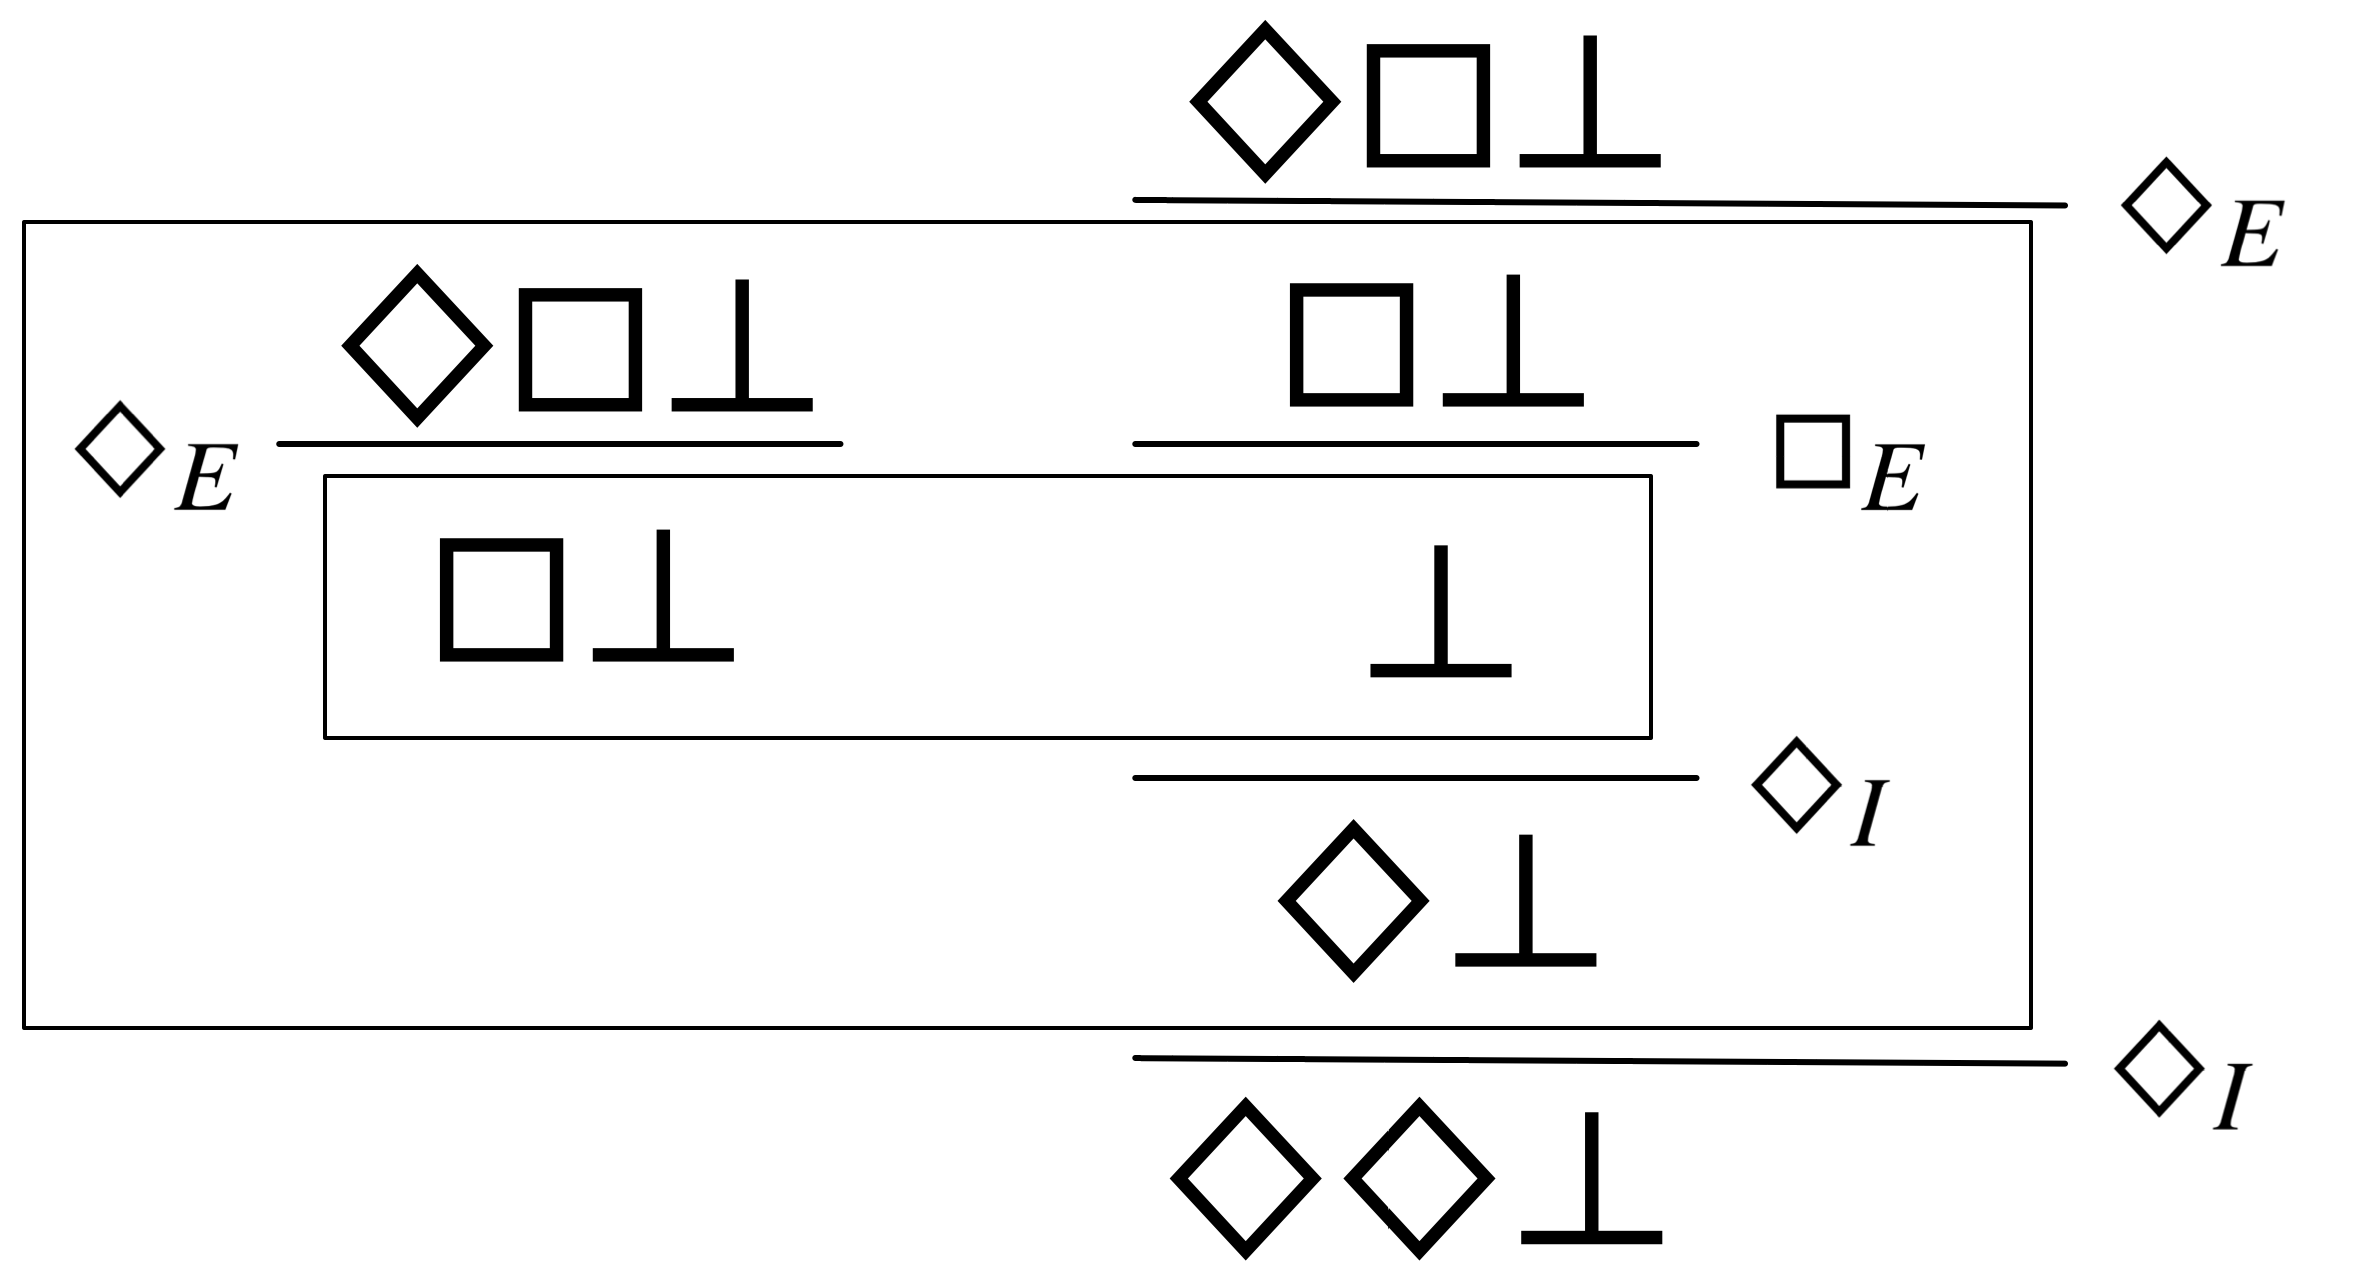
\includegraphics[width=0.4\textwidth]{Derivation}
\end{center}
%\smallskip

% $$
% \infer[\pos_I]{\pos \pos \bot}{
% \infer[\pos_I]{\pos \bot}{  
% \infer[\nec_E]{\bot}{
% \infer[\pos_E]{\nec \bot}{
%   \pos \nec \bot
% }
% }
% }
% }
% $$
\end{enumerate}

\end{enumerate}

An interesting and unusual feature of the derivation shown above is that the leftmost $\pos_E$ (diamond elimination) inference derives a formula ($\nec \bot$) that is never used as a premise. This is necessary because of the \emph{eigen-box} condition, which requires that every box must be accessed by exactly one \emph{strong} modal rule. The purpose of the \emph{strong} $\pos_E$ inference is merely to create and access the innermost box that is needed by the \emph{weak} $\nec_E$ and $\pos_I$ inferences inside the outermost box.

The proofs above have been formalized and verified step-by-step in \textsc{Coq}. The complete proofs can be found in \url{https://github.com/FormalTheology/GoedelGod}. The following \textsc{Coq} script shows the formalization of step 8 of the meta-logic proof.


\begin{Verbatim}[frame=single,commandchars=\\\{\},fontsize=\verbsize]
\Lemma dia_box_false_to_false_meta: [(dia (box mFalse))] -> [mFalse].
\Proof. intro H. intro w.
destruct (H w) as [w0 [R0 H0]]. destruct (H w0) as [w1 [R1 H1]].
box_elim H0 w1 HF. unfold mFalse in HF. destruct HF as [p [HF1 HF2]].
contradiction. \Qed.
\end{Verbatim}


\noindent
The other \textsc{Coq} scripts below show the formalization of step 8\textsuperscript{*} of the object-logic proof.

\begin{Verbatim}[frame=single,commandchars=\\\{\},fontsize=\verbsize]
\Lemma mimplies_to_mnot: [mforall p:o, (p m-> mFalse) m-> (m~ p)].
\Proof. mv. intro p. intro H. intro H0. 
destruct (H H0) as [p0 [H1 H2]]. apply H2. exact H1. \Qed.

\Lemma dia_not_not_box: [ mforall p, (dia (m~ p)) m-> (m~ (box p)) ].
\Proof. mv. intro p. intro H1. intro H2. 
dia_e H1. apply H. box_e H2 H3. exact H3. \Qed.

\Lemma dia_box_false_to_false_object: [(dia (box mFalse))] -> [mFalse].
\Proof. intro H. intro w. exists (dia (dia mFalse)).
split.
  dia_e (H w). dia_e (H w0). dia_i w0. dia_i w1. box_e H0 H3. exact H3.

  apply box_not_not_dia. box_i. apply box_not_not_dia. box_i.
  apply mimplies_to_mnot. intro H4. exact H4. \Qed.
\end{Verbatim}

\noindent
Due to a deliberate and disciplined use of only 
the simplest (and non-automatic) \textsc{Coq} tactics, 
there is a straightforward correspondence between the tactics used 
in the scripts above and the inference rules of the modal natural 
deduction calculus \cite{CSR}. Therefore, the lengths of the proof 
scripts (in number of tactic applications) can serve as estimations 
for the lengths of the corresponding natural deduction proof. 
It is noticeable that the meta-logic proof is significantly shorter 
than the pure object-logic proof. An in-depth analysis 
reveals that the reasoning about the possible worlds semantics in 
the meta-logic proof acts as a short-cut: when it becomes impossible (in step 8) to build the third world $w'$ (because $\bot$ would have to hold in it, and thus $w'$ would be contradictory), a contradiction at the HOL level can be immediately derived, completing the proof. In the object-level proof, on the other hand, such a contradiction had to be found in the arbitrary initial world $w$. This not only requires additional tedious logical inferences (cf. the proofs of the lemmas \texttt{mimplies\_to\_mnot} and \texttt{dia\_not\_not\_box}), but also a non-trivial guessing of the instantiating contradictory proposition $\pos \pos \bot$, whose purpose is precisely to carry over the contradiction from $w'$ back to $w$.



\section{Conclusion}\label{sec:conclusion}


The axioms and definitions in G\"odel's manuscript are inconsistent (even in the weakest modal logic \K);
this was detected automatically by the prover
\textsc{Leo-II}. In our previous work \cite{C55}, we presented a human-readable and intuitive meta-logic explanation for the inconsistency, and we formalized and semi-automatically reconstructed it in the \textsc{Isabelle} proof assistant. Here this work was extended with an object-level explanation, and both explanations were formalized step-by-step in \textsc{Coq} proof assistant. A comparison of the formal \textsc{Coq} proofs of both explanations revealed that the meta-logic reasoning is more powerful, because it enables shortcuts and, therefore, requires fewer inferences and guesses. We conjecture that this is not accidental, but rather a fundamental reason why the embedding approach is effective in practice. 

It is kind of entertaining that our work reveals a mistake in
G\"odel's manuscript and at same time further substantiates G\"odel's
belief that ``there is a scientific (exact) philosophy and theology,
which deals with concepts of the highest abstractness; and this is
also most highly fruitful for science.''
\cite{Wang1996}[p. 316]. Indeed, through the investigation of
G\"odel's mistake, we have been led to an interesting little
conjecture in automated reasoning and proof theory (the global axiom
$\pos \nec \bot$ is inconsistent).



\bibliographystyle{plain}
\bibliography{Bibliography}



\end{document}

